\documentclass[twoside,a4paper]{article}
\usepackage{amsmath}
\usepackage{amsfonts}
%\usepackage{mathabx} %for the \wdcheck
\usepackage{amssymb}
\usepackage[labelfont=bf]{caption}
\usepackage[english]{babel}
\usepackage{bibgerm}
\usepackage[utf8]{inputenc}
\usepackage[OT1]{fontenc}
\usepackage{graphicx}
\usepackage{latexsym}
\usepackage{subcaption} 
\usepackage[inner=36pt, textwidth=345pt]{geometry}
\usepackage{subfiles}
\usepackage{siunitx}
\usepackage{tikz}
\usepackage{tikz-feynman}
\usepackage{ifthen} % for the tikz loops
\usepackage[toc,page]{appendix}
\usetikzlibrary{shapes.geometric}
\usetikzlibrary{decorations.pathmorphing}
\usepackage{twemojis}
\usepackage{hyperref}
\usepackage[makeroom]{cancel}
\usepackage{pdfpages}
\usepackage{bm}
\usepackage{layout}
\usepackage{ relsize }
\usepackage{float}
\usepackage{cancel}
\usepackage{stmaryrd}
\usepackage{TamwynLatexLib}
\usepackage{fancyhdr}
\usepackage[explicit]{titlesec}   
\usepackage{mathtools}
\usepackage{pgfplots}
\pgfplotsset{width=10cm,compat=1.9}
\usepackage{pdfpages}
\usepackage{bbm} %for the \mathbb{1}
\newcommand{\indc}{\mathlarger{\mathlarger{\mathbbm{1}\normalsize}}}

\usepackage[style=numeric, sorting=none]{biblatex} %backend=biber, sortlocale=en_EN
\addbibresource{references.bib}

%\input{C:/Users/Tamwyn/Documents/CustomLatexTextMF/mytexmf/tex/latex/UniLaTeXPackage/Arto/ArtoMain.tex}


\geometry{ 
    bindingoffset=1.0471975512cm, 
    left=2.9cm, 
    right=2.6cm, 
    top=1.6cm, 
    bottom=2.5cm
}

\renewcommand{\footnoterule}{%
    \vspace*{-3pt} % Vertical space before the line
    
\begin{tikzpicture}
        \coordinate (A) at (0.2\textwidth,-0.5);
        \coordinate (B) at (0,-0.5);
        \draw[black, line width = 0.5pt] (B) -- (A);
        \draw ($(A) + (0.1,0 )$) rectangle ++(0.1,0.1);
        \draw ($(B) - (0.3,0 )$) rectangle ++(0.2,0.2);
    \end{tikzpicture}

    \vspace*{3pt} % Vertical space after the line
}
%\thispagestyle{empty}
% \setlength\parindent{0pt}
\pagestyle{fancy}
\fancyhf{} % Clear default header and footer
% Customize footer with design around the page number
\fancyfoot[C]{
    \begin{tikzpicture}[baseline=(X.base)]
        \node (X) at (0,0) [] {\thepage};
        \coordinate (A) at ($(X.north west) + (-0.1,-0.2)$);
        \coordinate (A2) at ($(X.north west) + (-0.5,-0.2)$);
        \coordinate (A3) at ($(X.north west) + (-0.6,-0.2)$);
        \coordinate (B) at ($(X.north east) + (0.1,-0.2)$);
        \coordinate (B2) at ($(X.north east) + (+0.5, -0.2)$);
        \coordinate (B3) at ($(X.north east) + (+0.6, -0.2)$);
        \coordinate (C) at ($(X.south east) + (0.1,0.15)$);
        \coordinate (C2) at ($(X.south east) + (0.2,0.15)$);
        \coordinate (D) at ($(X.south west) + (-0.1,0.15)$);
        \coordinate (D2) at ($(X.south west) + (-0.2,0.15)$);

        \draw (A) -- (A2);
        \draw (B) -- (B2);
        \draw (C) -- (C2);
        \draw (D) -- (D2);
        \draw (A3) rectangle ++(-0.1,0.1);
        \draw (B3) rectangle ++(0.1,0.1);
    \end{tikzpicture}
}
\renewcommand{\headrulewidth}{0pt}
\DeclareSIUnit{\site}{\text{site}}
% Define a custom macro for the equation with a condition

% \pgfmathdeclarefunction{ifthenelsefpu}{3}{%
%   \pgfmathparse{#1*#2 + !#1*#3}%
% }

\pgfmathdeclarefunction{ifthenelsefpu}{3}{%
  \pgfmathparse{#1 == 1 ? #2 : #3}%
}
% \pgfmathdeclarefunction{f}{3}{%
% \pgfmathparse{ifthenelse(abs(cos(#1-pi) + cos(#2-pi) - (#3/2)) < 1,  #3, nan)}%
% }
\pgfmathdeclarefunction{f}{3}{%
  \pgfmathparse{ifthenelse(abs(cos(deg(#1-pi)) + cos(deg(#2-pi)) - (#3/2)) < 5e-2,  #3/2 , nan)}%
}
% Define the function fd
\pgfmathdeclarefunction{fd}{1}{%
  \pgfmathparse{ifthenelse(#1 < 1e-3, #1/2, nan)}%
}


% \pgfmathdeclarefunction{g}{1}{%
%   \pgflibraryfpuifactive{%
%     \pgfkeys{/pgf/fpu=false}%
%     \pgfmathfloattofixed{#1}%
%     \let\x=\pgfmathresult%
%   }%
%   {%
%     \pgfmathparse{#1}%
%     \let\x=\pgfmathresult%
%   }%
%   \pgfmathparse{ifthenelse(\x<0,(\x)^2,\x)}%
% }

% Optional: Adjust spacing before/after sections
\titlespacing*{\section}{0pt}{1em}{1em}

% Temporarily disable custom formatting when including subfiles


\begin{document}
\definecolor{TamGreen}{HTML}{00C4F6}
\definecolor{TamTangerine}{HTML}{325BCB}
\definecolor{TamDarkBlue}{HTML}{666A86}
\definecolor{TamDarkBlue2}{HTML}{788AA3}
\definecolor{TamLightGreen}{HTML}{92B6B1}
\definecolor{TamLightGY}{HTML}{B2C9AB}
\definecolor{TamYellow}{HTML}{E8DDB5}
\definecolor{Brillou1}{HTML}{2D70B3}
\definecolor{Brillou2}{HTML}{3D8F4A}
\definecolor{Brillou3}{HTML}{FA7E19}
\definecolor{Brillou4}{HTML}{C74440}

\newcommand{\rem}[1]{\textcolor{TamGreen}{#1}}
\thispagestyle{empty}
% 
\includepdf[pages=-]{Ressources/Title.pdf} 
% \newpage
\thispagestyle{empty}
\begin{center} 
    \noindent\Huge.\\
    \noindent$\circ$\\
    \rule{0.1\textwidth}{0.75pt}\\
    \rule[20pt]{0.17\textwidth}{0.75pt} \rule[20pt]{0.5\textwidth}{0.75pt} \rule[20pt]{0.17\textwidth}{0.75pt}\\
    \vspace*{30pt}
    \Huge $\mathcal{P}$\textit{roximity} $\mathcal{E}$\textit{ffects}\\
     \textit{in}\\ 
    $\mathcal{A}$\textit{ltermagnetic}  $\mathcal{S}$\textit{ystems}
    \vspace*{12pt}\\
    $~\sim\circ\sim~$
    \vspace*{48pt}\\
    \normalsize
 a bachelor thesis.\\

\end{center}
\vspace*{60pt}
\noindent
\normalsize
\textbf{Written by} Arto Steffan, \\
\textbf{under the supervision of} Prof. Dr. Jacob Wüsthoff Linder, \\
\textbf{and corrected by} Prof. Dr. Wolfgang Belzig.\\
\vspace*{112pt}
\begin{center}
    February 3rd, 2025
\end{center}
\vspace*{12pt}
\begin{center}
    \rule{.4\textwidth}{0.4pt}
\end{center}
\vspace*{12pt}
\begin{figure}[H]
    \centering
    \begin{subfigure}{0.45\textwidth}
        
\includegraphics[width=.8\textwidth]{Ressources/UniKn.png}
    \end{subfigure}\hspace*{0.1\textwidth}
    \begin{subfigure}{0.45\textwidth}
        
\includegraphics[width=0.9\textwidth]{Ressources/ntnu.png}
        \vspace*{12pt}
    \end{subfigure}
\end{figure}


\newpage
% \shipout\null
\subfile{Pages/0_Acknolegmend.tex} 
\vspace*{7pt}

\newpage
% \shipout\null

% -----------------------------------------------------------
% Content prepartion

    \tableofcontents
    \thispagestyle{empty}	
    
\newpage
% \shipout\null
    \setcounter{page}{1}
    \pagenumbering{arabic}



% -----------------------------------------------------------
% Redefine the \section{} command to include the label
\titleformat{\section}[hang]
{\LARGE\bfseries} {} {0pt} {%
  \begin{tikzpicture}[baseline=(Educ.base)]
    \node[inner sep=0pt, anchor=west, align=left, ,text width=13.75cm] (Educ) at (0,0) {\thesection \hspace*{0.3em} #1};;
    \coordinate (A) at ($(Educ.south) + (1.35, -0.45)$);
    \draw[thick] ($(Educ.south west) + (0.1, -0.7)$) rectangle ++(-0.4,0.4);
    \draw[thick] (A) rectangle ++(-0.15,0.15);
    \draw[-, thick] ($(Educ.south west) + (0.4, -0.3)$) -- ($(Educ.south) + (1, -0.3)$);
    \draw[thick] ($(Educ.east) + (0, -0.075)$) rectangle ++(-0.15,0.15);
    \draw[-, thick] ($(Educ.east) + (-0.2, 0)$) -- ($(Educ.east) + (-0.35, 0)$);
    \draw[-, thick] ($(Educ.east) + (-0.075, -0.15)$) -- ($(Educ.east) + (-0.075, -0.4)$);
    \draw[-, thin] ($(Educ.east) + (-0.2,-0.125)$) -- ($(Educ.east) + (-0.3, -0.2)$);
    % \draw[-, thin] ($(Educ.east) + (-0.2,0.125)$) -- ($(Educ.east) + (-0.275, 0.175)$);
    \draw[-, thin] ($(Educ.east) + (-0.2,-0.125)+ (0.45,.4)$) -- ($(Educ.east)+ (-0.325, -0.225) + (.4,.35)$);
 \end{tikzpicture}
}
\newpage
\subfile{Pages/1_Introduction.tex}
\newpage
\subfile{Pages/2_TheoreticalBackground.tex} 
\newpage
\subfile{Pages/6_Altermagnetism.tex}
\newpage
\subfile{Pages/3_BdGFormalism.tex}
\subfile{Pages/7_CurrentsInLattice.tex}
\newpage
\subfile{Pages/5_Simulations.tex} 
\subfile{Pages/4_Results.tex}
\newpage
\begin{appendices}
    \subfile{Pages/8_AdvancedSupercond.tex}
\end{appendices}

%-----------------------------------------------------------
% Credits
\titleformat{\section}{\normalfont\Large\bfseries}{\thesection \hspace*{0.3em} #1}{1em}{}

\newpage
    \subfile{Pages/Literature.tex}
\newpage
% 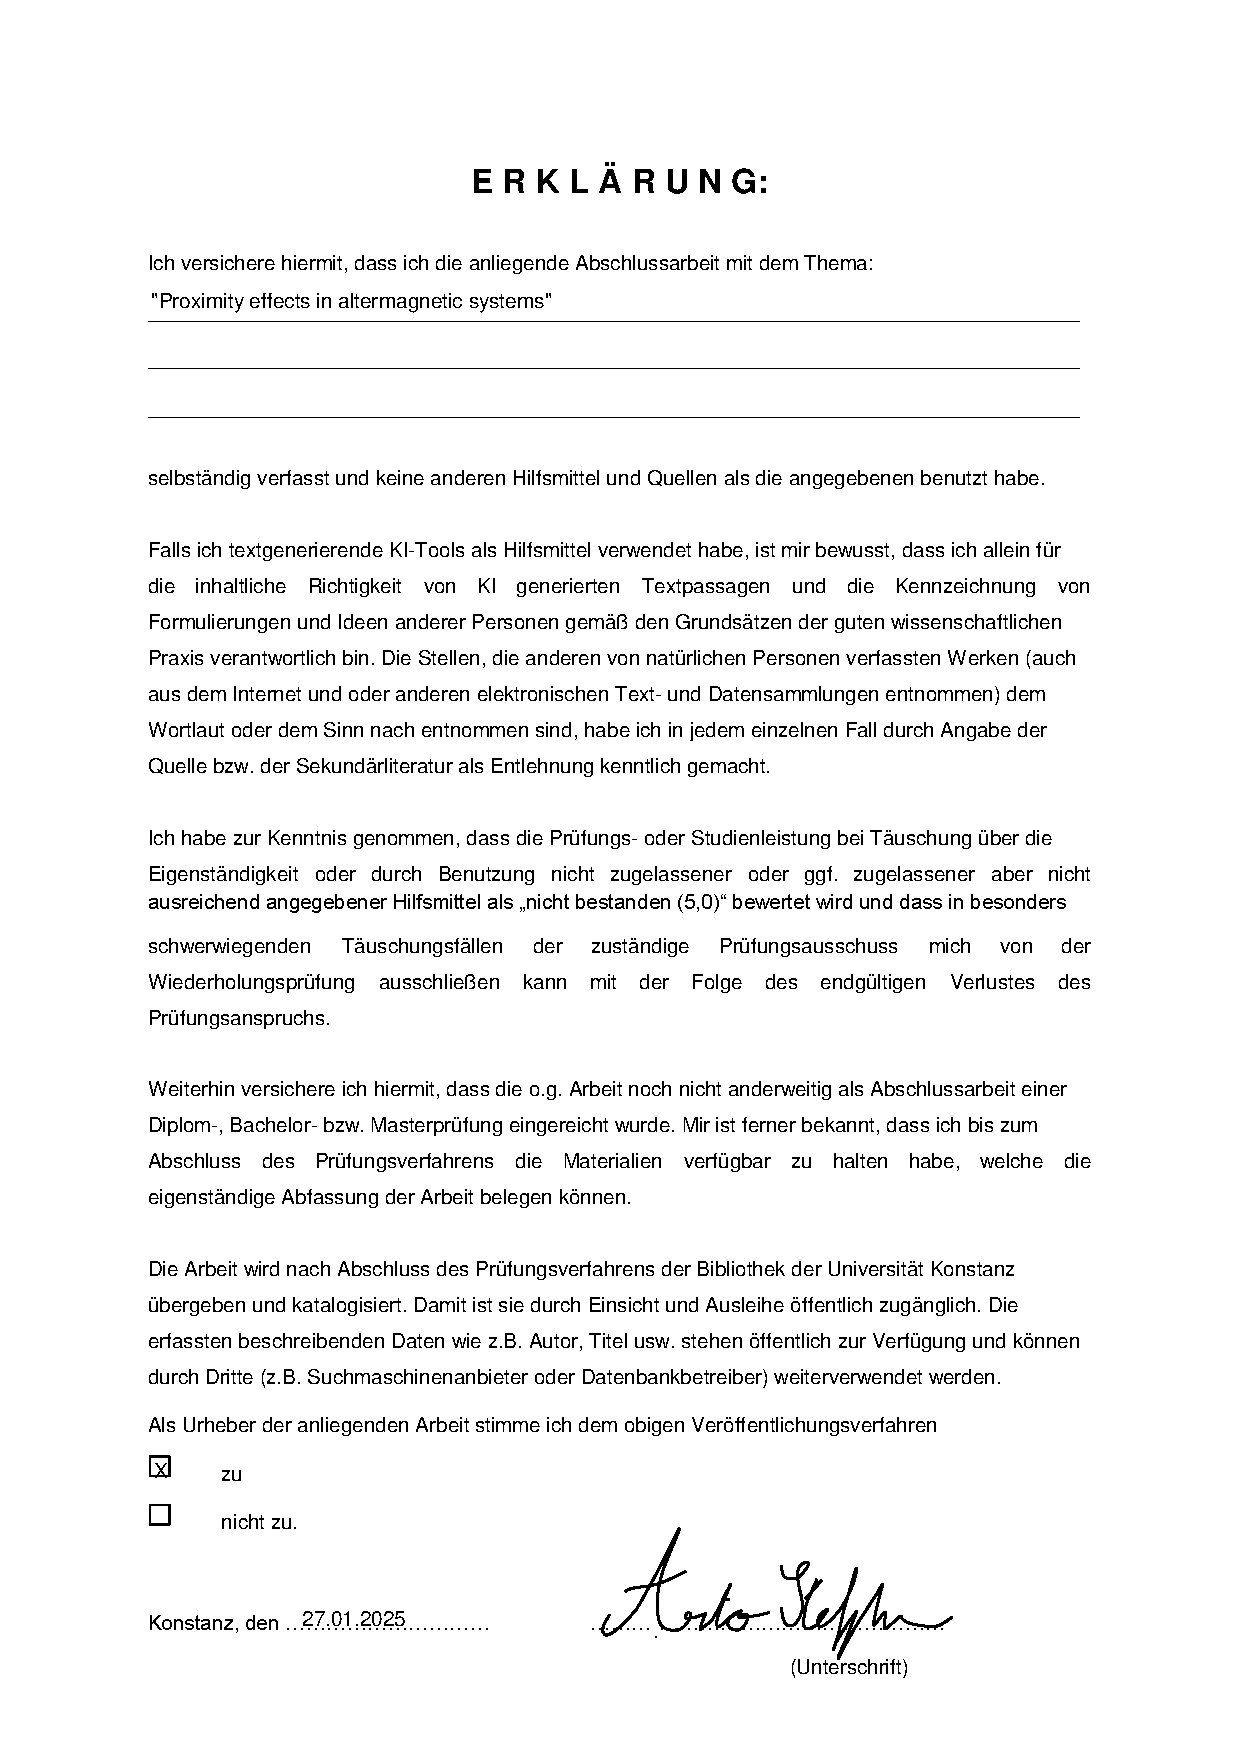
\includepdf[pages=-]{Ressources/Eigenstaendigkeitserklearung3.pdf}
% \includepdf[pages=-]{Ressources/Themenzuteilung Steffan 1 Gutachter mit Verlängerung.pdf}
\vspace*{150pt}
\thispagestyle{empty}

\begin{center}
    

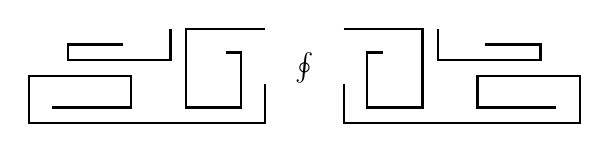
\begin{tikzpicture}
    \coordinate (A) at (0,0);
  
    \coordinate (B) at (0.5, 0.5);
    \coordinate (C) at (1.5, 0.5);
    \coordinate (D) at (1.5, -0.5);
    \coordinate (E) at (0.8, -0.5);
    \coordinate (F) at (0.8, 0.2);
    \coordinate (G) at (1, 0.2);
  
    \coordinate (H) at (0.5, -0.2);
    \coordinate (I) at (0.5, -0.7);
    \coordinate (J) at (3.5, -0.7);
    \coordinate (K) at (3.5, -0.1);
    \coordinate (L) at (2.2, -0.1);
    \coordinate (M) at (2.2, -0.5);
    \coordinate (N) at (3.2, -0.5);
  
    \coordinate (S) at (1.7, 0.5);
    \coordinate (O) at (1.7, 0.1);
    \coordinate (P) at (3, 0.1);
    \coordinate (Q) at (3, 0.3);
    \coordinate (R) at (2.3, 0.3);
  
    \draw[thick] (B) -- (C) -- (D) -- (E) -- (F) -- (G);  
    \draw[thick] (H) -- (I) -- (J) -- (K) -- (L)-- (M) -- (N);  
    \draw[thick] (S) -- (O) -- (P) -- (Q) -- (R);
  
    \node[] at (A) {\(\oint\)};
  
    \coordinate (-B) at (-0.5, 0.5);
    \coordinate (-C) at (-1.5, 0.5);
    \coordinate (-D) at (-1.5, -0.5);
    \coordinate (-E) at (-0.8, -0.5);
    \coordinate (-F) at (-0.8, 0.2);
    \coordinate (-G) at (-1, 0.2);
  
    \coordinate (-H) at (-0.5, -0.2);
    \coordinate (-I) at (-0.5, -0.7);
    \coordinate (-J) at (-3.5, -0.7);
    \coordinate (-K) at (-3.5, -0.1);
    \coordinate (-L) at (-2.2, -0.1);
    \coordinate (-M) at (-2.2, -0.5);
    \coordinate (-N) at (-3.2, -0.5);
  
    \coordinate (-S) at (-1.7, 0.5);
    \coordinate (-O) at (-1.7, 0.1);
    \coordinate (-P) at (-3, 0.1);
    \coordinate (-Q) at (-3, 0.3);
    \coordinate (-R) at (-2.3, 0.3);
  
    \draw[thick] (-B) -- (-C) -- (-D) -- (-E) -- (-F) -- (-G);  
    \draw[thick] (-H) -- (-I) -- (-J) -- (-K) -- (-L)-- (-M) -- (-N);  
    \draw[thick] (-S) -- (-O) -- (-P) -- (-Q) -- (-R);
  
   \end{tikzpicture}
\end{center}
\end{document}